\documentclass[border=3pt]{standalone}
% Shared TikZ styles for the Ch. 3–8 diagrams (standalone PDFs); extends the Ch. 1 palette (s1_vs_llm_common.tex).
\usepackage[T1]{fontenc}
\usepackage{lmodern}
\usepackage[english]{babel}
\usepackage{amsmath,amssymb}
\usepackage{tikz}
\usetikzlibrary{shapes.geometric,shapes.misc,positioning,fit,arrows.meta,calc,backgrounds,decorations.pathreplacing,patterns}
\definecolor{ioFill}{HTML}{F1F0EC}\definecolor{ioLine}{HTML}{52514E}
\definecolor{modFill}{HTML}{E8F1FB}\definecolor{modLine}{HTML}{2A78D6}
\definecolor{decFill}{HTML}{ECE9F7}\definecolor{decLine}{HTML}{4A3AA7}
\definecolor{postFill}{HTML}{FFF6E0}\definecolor{postLine}{HTML}{EDA100}
\definecolor{okFill}{HTML}{EAF7F1}\definecolor{okLine}{HTML}{1BAF7A}
\definecolor{badFill}{HTML}{FDECEC}\definecolor{badLine}{HTML}{E34948}
\definecolor{nmFill}{HTML}{EFEAF8}\definecolor{nmLine}{HTML}{4A3AA7}
\definecolor{loopRed}{HTML}{E34948}\definecolor{clusterLine}{HTML}{9A9890}\definecolor{ink2}{HTML}{52514E}
\definecolor{orangeA}{HTML}{EB6834}
\tikzset{
  every node/.style={font=\small, align=center},
  io/.style={trapezium, trapezium left angle=72, trapezium right angle=108, trapezium stretches body,
             draw=ioLine, fill=ioFill, thick, inner sep=3pt, minimum height=2.4em},
  model/.style={rectangle, draw=modLine, fill=modFill, very thick, inner sep=4pt, minimum height=2.4em, text width=#1},
  model/.default=3.6cm,
  post/.style={rectangle, draw=postLine, fill=postFill, very thick, inner sep=4pt, minimum height=2.2em, text width=#1},
  post/.default=3.6cm,
  data/.style={cylinder, shape border rotate=90, aspect=0.18, draw=okLine, fill=okFill, very thick, inner sep=3pt, minimum height=2.6em, text width=#1},
  data/.default=2.4cm,
  decision/.style={diamond, aspect=2.1, draw=decLine, fill=decFill, very thick, inner sep=1pt},
  outcome/.style={rounded rectangle, draw=#1, thick, inner sep=4pt, minimum height=2em},
  arrow/.style={-{Latex[length=2mm]}, thick, ioLine},
  dashedarrow/.style={-{Latex[length=2mm]}, thick, ioLine, dashed},
  loop/.style={-{Latex[length=2.4mm]}, line width=1.4pt, loopRed},
  cluster/.style={draw=clusterLine, dashed, rounded corners=3pt, inner sep=7pt},
  clusterlabel/.style={font=\small\bfseries, text=ioLine},
  note/.style={font=\footnotesize, text=ink2},
  tok/.style={rectangle, draw=ioLine, fill=ioFill, thin, inner sep=2pt, minimum height=1.6em, font=\footnotesize},
  vmark/.style={rectangle, draw=orangeA, fill=postFill, thick, inner sep=2pt, minimum height=1.6em, font=\footnotesize\ttfamily},
}

\begin{document}
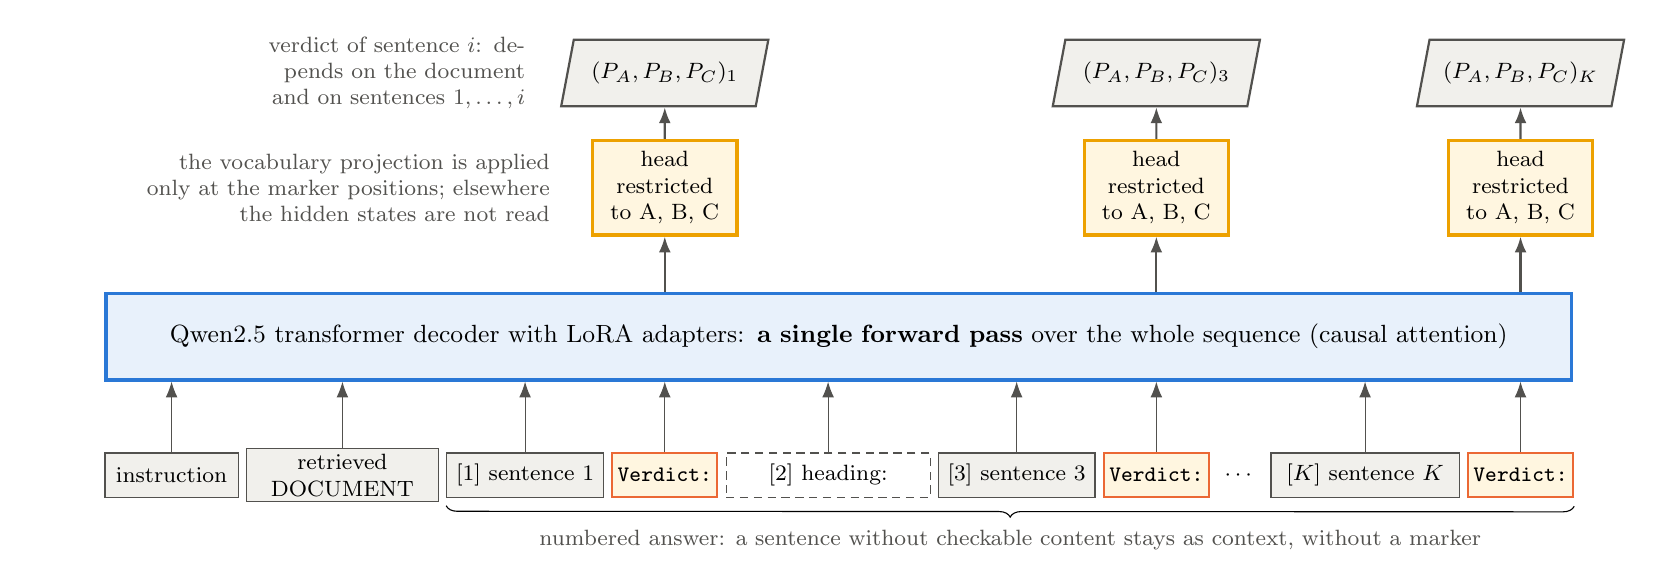
\begin{tikzpicture}[node distance=0.9mm]
  % token sequence
  \node[tok, text width=1.55cm] (ins) {instruction};
  \node[tok, right=of ins, text width=2.3cm] (doc) {retrieved\\DOCUMENT};
  \node[tok, right=of doc, text width=1.85cm] (s1) {[1] sentence 1};
  \node[vmark, right=of s1] (m1) {Verdict:};
  \node[tok, right=of m1, text width=2.45cm, fill=white, densely dashed] (s2) {[2] heading:};
  \node[tok, right=of s2, text width=1.85cm] (s3) {[3] sentence 3};
  \node[vmark, right=of s3] (m3) {Verdict:};
  \node[right=0.6mm of m3, font=\footnotesize] (dots) {$\cdots$};
  \node[tok, right=0.6mm of dots, text width=2.25cm] (sk) {[$K$] sentence $K$};
  \node[vmark, right=of sk] (mk) {Verdict:};
  \draw[decorate, decoration={brace, amplitude=4pt, mirror}] ([yshift=-1mm]s1.south west) -- node[below=5pt, note] {numbered answer: a sentence without checkable content stays as context, without a marker} ([yshift=-1mm]mk.south east);
  % transformer
  \path let \p1=(ins.west), \p2=(mk.east) in node[model=\x2-\x1-8pt-1.6pt, minimum height=1.1cm, anchor=south west] (tr) at ([yshift=9mm]ins.north west) {Qwen2.5 transformer decoder with LoRA adapters: \textbf{a single forward pass} over the whole sequence (causal attention)};
  \foreach \n in {ins,doc,s1,m1,s2,s3,m3,sk,mk} \draw[arrow, thin] (\n.north) -- (\n.north |- tr.south);
  % heads only at markers
  \foreach \n/\k in {m1/1,m3/3,mk/K} {
    \node[post=1.55cm, above=7mm of \n.north |- tr.north, font=\footnotesize] (h\k) {head restricted\\to A, B, C};
    \draw[arrow] (\n.north |- tr.north) -- (h\k);
    \node[io, above=4mm of h\k, font=\footnotesize, text width=2.1cm] (o\k) {$(P_A, P_B, P_C)_{\k}$};
    \draw[arrow] (h\k) -- (o\k);
  }
  \node[note, anchor=east, align=right, text width=6.2cm] at ([xshift=-4mm]h1.west |- h1) {the vocabulary projection is applied\\only at the marker positions; elsewhere\\the hidden states are not read};
  \node[note, anchor=east, align=right, text width=6.2cm] at ([xshift=-4mm]o1.west |- o1) {verdict of sentence $i$: depends on the document\\and on sentences $1,\dots,i$};
\end{tikzpicture}
\end{document}
